\documentclass[11pt,a4paper]{article}

% ----------------------------- PACKAGES -----------------------------
\usepackage[margin=1in]{geometry}
\usepackage{amsmath,amssymb}
\usepackage{tikz}
\usetikzlibrary{arrows.meta,positioning,shapes.geometric,fit,backgrounds,calc,decorations.pathreplacing}
\usepackage{booktabs}
\usepackage{array}
\usepackage{xcolor}
\usepackage{listings}
\usepackage{enumitem}
\usepackage{hyperref}
\usepackage{caption}
\usepackage{tcolorbox}
\tcbuselibrary{skins,breakable}
\usepackage{fancyhdr}
\usepackage{titlesec}
\usepackage{parskip}

% ----------------------------- COLORS -----------------------------
\definecolor{navyblue}{RGB}{25,55,95}
\definecolor{softblue}{RGB}{214,229,247}
\definecolor{softgreen}{RGB}{219,242,224}
\definecolor{softred}{RGB}{250,220,220}
\definecolor{softyellow}{RGB}{255,244,214}
\definecolor{softgray}{RGB}{235,235,235}
\definecolor{codebg}{RGB}{246,246,246}

% ----------------------------- LISTINGS -----------------------------
\lstdefinestyle{codeblock}{
  backgroundcolor=\color{codebg},
  basicstyle=\ttfamily\small,
  breaklines=true,
  frame=single,
  rulecolor=\color{softgray},
  framerule=0.5pt,
  xleftmargin=4pt,
  xrightmargin=4pt,
  columns=fullflexible,
  keepspaces=true,
}
\lstset{style=codeblock}

% ----------------------------- SECTION STYLE -----------------------------
\titleformat{\section}{\Large\bfseries\color{navyblue}}{\thesection}{0.6em}{}
\titleformat{\subsection}{\large\bfseries\color{navyblue}}{\thesubsection}{0.6em}{}
\titleformat{\subsubsection}{\bfseries\color{navyblue}}{\thesubsubsection}{0.6em}{}

\pagestyle{fancy}
\fancyhf{}
\fancyhead[L]{\small SafeNav-LLM: Architectural Deep Dive}
\fancyhead[R]{\small\thepage}
\renewcommand{\headrulewidth}{0.4pt}

% ----------------------------- TIKZ STYLES -----------------------------
\tikzset{
  block/.style={rectangle, rounded corners, draw=navyblue, thick, fill=softblue,
                minimum width=2.6cm, minimum height=0.9cm, align=center, font=\small},
  blockgreen/.style={block, fill=softgreen},
  blockred/.style={block, fill=softred},
  blockyellow/.style={block, fill=softyellow},
  blockgray/.style={block, fill=softgray, draw=gray},
  arrow/.style={-{Stealth[length=2.2mm]}, thick, navyblue},
  arrowred/.style={-{Stealth[length=2.2mm]}, thick, red!60!black},
  arrowgreen/.style={-{Stealth[length=2.2mm]}, thick, green!40!black},
  label/.style={font=\scriptsize\itshape, align=center},
}

\newcommand{\gapbox}[2]{%
  \begin{tcolorbox}[colback=softblue,colframe=navyblue,title={#1},fonttitle=\bfseries,breakable]
  #2
  \end{tcolorbox}%
}

\title{\vspace{-1.5cm}\textbf{SafeNav-LLM: A Layer-by-Layer Architectural Analysis}\\[0.3em]
\large On-Device Semantic Waypoint Resolution for Nav2}
\author{}
\date{}

% ============================================================================
\begin{document}
\maketitle
\thispagestyle{fancy}

\begin{abstract}
\noindent This document provides a layer-by-layer explanation of the SafeNav-LLM
architecture: an on-device, closed-vocabulary, Nav2-native language model
resolver for semantic navigation goals. The problem is not simply ``using an
LLM for navigation,'' but making semantic goal resolution safe, offline, and
native to Nav2. Four architectural gaps are examined in depth --- on-device
inference, closed-set structural safety, native BehaviorTree integration, and
deployment-calibrated confidence --- along with how they compose into a single
defense-in-depth system.
\end{abstract}

\tableofcontents
\newpage

% ============================================================================
\section{Understanding the Problem}
\label{sec:problem}

Before discussing the four gaps individually, it is necessary to understand
\emph{what exactly the system is replacing}. A conventional Nav2 robot expects
a metric pose, not a natural-language description of a place. Nav2 does not
inherently understand the semantic concept ``charging dock'' --- it understands
a coordinate frame.

\begin{figure}[h]
\centering
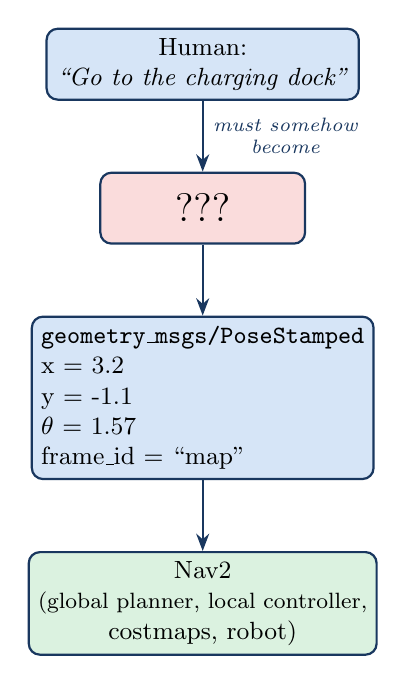
\begin{tikzpicture}[node distance=0.9cm]
\node[block] (human) {Human: \\ \textit{``Go to the charging dock''}};
\node[blockred, below=of human] (unknown) {\Large ???};
\node[block, below=0.9cm of unknown, align=left] (pose) {\texttt{geometry\_msgs/PoseStamped} \\ x = 3.2 \\ y = -1.1 \\ $\theta$ = 1.57 \\ frame\_id = ``map''};
\node[blockgreen, below=of pose] (nav2) {Nav2 \\ \footnotesize (global planner, local controller,\\ costmaps, robot)};

\draw[arrow] (human) -- (unknown) node[midway,right,label] {must somehow\\become};
\draw[arrow] (unknown) -- (pose);
\draw[arrow] (pose) -- (nav2);
\end{tikzpicture}
\caption{The core translation problem: Nav2 only understands metric poses, not named places.}
\end{figure}

SafeNav-LLM introduces a semantic layer that bridges this gap:

\begin{figure}[h]
\centering
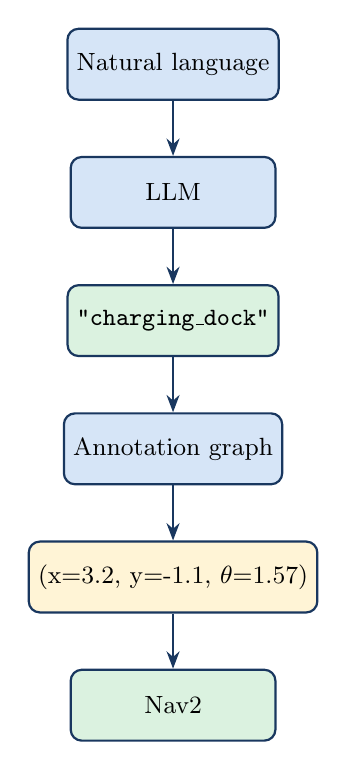
\begin{tikzpicture}[node distance=0.7cm]
\node[block] (nl) {Natural language};
\node[block, below=of nl] (llm) {LLM};
\node[blockgreen, below=of llm] (name) {\texttt{"charging\_dock"}};
\node[block, below=of name] (graph) {Annotation graph};
\node[blockyellow, below=of graph] (coords) {(x=3.2, y=-1.1, $\theta$=1.57)};
\node[blockgreen, below=of coords] (nav2b) {Nav2};

\foreach \a/\b in {nl/llm, llm/name, name/graph, graph/coords, coords/nav2b}
  \draw[arrow] (\a) -- (\b);
\end{tikzpicture}
\caption{The semantic waypoint resolution pipeline introduced by SafeNav-LLM.}
\end{figure}

The LLM sits between a messy human language space and a physical robot control
space, which is precisely why safety becomes the central engineering concern.

% ============================================================================
\section{Gap A --- Fully On-Device LLM Inference}
\label{sec:gapa}

\subsection{Cloud-Based Architecture and Its Dependencies}

A cloud-based architecture routes every command through the internet:

\begin{figure}[h]
\centering
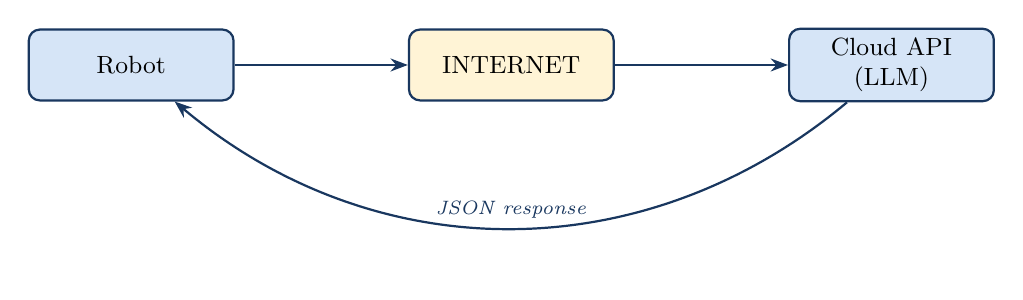
\begin{tikzpicture}[node distance=1.4cm and 2.2cm]
\node[block] (robot) {Robot};
\node[blockyellow, right=of robot] (internet) {INTERNET};
\node[block, right=of internet] (cloud) {Cloud API \\ (LLM)};

\draw[arrow] (robot) -- (internet);
\draw[arrow] (internet) -- (cloud);
\draw[arrow] (cloud) to[bend left=40] node[above,label] {JSON response} (robot);
\end{tikzpicture}
\caption{Cloud-based LLM resolution: convenient, but network-dependent.}
\end{figure}

\begin{lstlisting}[caption={Example cloud response for a resolved room}]
{
    "room": "server_room",
    "confidence": 0.91
}
\end{lstlisting}

This convenience creates three coupled dependencies, illustrated below.

\begin{figure}[h]
\centering
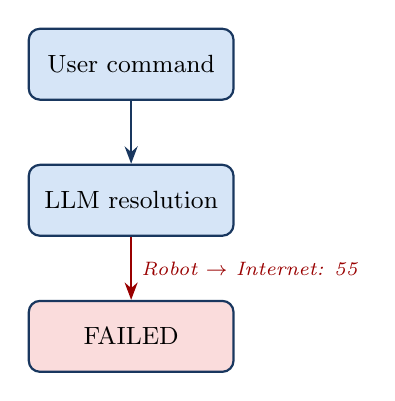
\begin{tikzpicture}[node distance=0.8cm]
\node[block] (cmd) {User command};
\node[block, below=of cmd] (res) {LLM resolution};
\node[blockred, below=of res] (fail) {FAILED};
\draw[arrow] (cmd) -- (res);
\draw[arrowred] (res) -- node[right,label]{Robot $\to$ Internet: \ding{55}} (fail);
\end{tikzpicture}
\caption{Connectivity dependency: no network means no semantic resolution.}
\end{figure}

The design target environments --- hospitals, factory floors, cleanrooms, and
secure research facilities --- may not permit outbound internet access at all.
The requirement is therefore that \emph{the robot must possess everything
necessary to perform semantic resolution locally.}

\subsection{Privacy Dependency}

\begin{figure}[h]
\centering
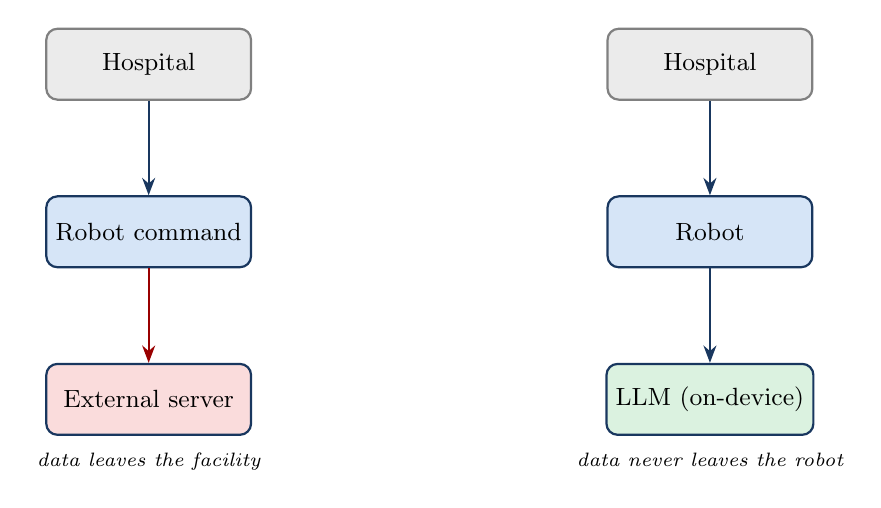
\begin{tikzpicture}[node distance=1.2cm and 2.2cm]
% Left: cloud case
\node[blockgray] (hosp1) {Hospital};
\node[block, below=of hosp1] (robot1) {Robot command};
\node[blockred, below=of robot1] (ext) {External server};
\draw[arrow] (hosp1) -- (robot1);
\draw[arrowred] (robot1) -- (ext);
\node[label, below=0.1cm of ext] {data leaves the facility};

% Right: local case
\node[blockgray, right=4.5cm of hosp1] (hosp2) {Hospital};
\node[block, below=of hosp2] (robot2) {Robot};
\node[blockgreen, below=of robot2] (llm2) {LLM (on-device)};
\draw[arrow] (hosp2) -- (robot2);
\draw[arrow] (robot2) -- (llm2);
\node[label, below=0.1cm of llm2] {data never leaves the robot};
\end{tikzpicture}
\caption{Cloud inference introduces a data-flow boundary outside the facility (left); local inference keeps commands entirely on the robot (right).}
\end{figure}

Even commands without personal names can leak sensitive facility information:
building layout, room names, operational procedures, and restricted-area
identifiers. Local inference eliminates this exposure entirely.

\subsection{Latency Variability}

Cloud inference latency is not simply the LLM's compute time; it is the sum of
network upload, server queueing, LLM inference, and network download:

\[
\text{Total latency} = \underbrace{t_{\text{up}}}_{\text{network}} + \underbrace{t_{\text{queue}}}_{\text{server}} + \underbrace{t_{\text{LLM}}}_{\text{inference}} + \underbrace{t_{\text{down}}}_{\text{network}}
\]

\begin{table}[h]
\centering
\begin{tabular}{lc}
\toprule
\textbf{Request} & \textbf{Observed latency} \\
\midrule
Request 1 & 800\,ms \\
Request 2 & 1.4\,s \\
Request 3 & 3.7\,s \\
Request 4 & timeout \\
\bottomrule
\end{tabular}
\caption{Illustrative variability of cloud round-trip latency across requests.}
\end{table}

This unpredictability is particularly undesirable inside a BehaviorTree, which
motivates a local model together with an explicit \texttt{timeout\_ms} and a
target p90 hardware latency of $\leq 3$ seconds.

\subsection{Monetary Dependency}

Cloud LLM calls scale linearly with usage:
\[
\text{Annual API calls} \approx 10\ \tfrac{\text{cmds}}{\text{hr}} \times 8\ \tfrac{\text{hr}}{\text{day}} \times 300\ \text{days} = 24{,}000 \text{ calls/year}
\]
whereas on-device inference trades network/API cost for a one-time hardware
cost plus electricity and maintenance. This is a practical, not purely
scientific, deployment consideration.

\subsection{Fitting a Model on an Embedded System}

The robot's Jetson Orin NX has finite RAM, VRAM/shared memory, compute,
thermal budget, and power budget. A small model is therefore selected and
quantized:

\begin{figure}[h]
\centering
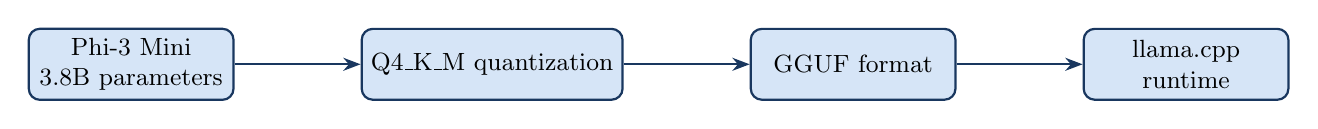
\begin{tikzpicture}[node distance=0.5cm]
\node[block] (m1) {Phi-3 Mini \\ 3.8B parameters};
\node[block, right=1.6cm of m1] (m2) {Q4\_K\_M quantization};
\node[block, right=1.6cm of m2] (m3) {GGUF format};
\node[block, right=1.6cm of m3] (m4) {llama.cpp \\ runtime};
\foreach \a/\b in {m1/m2, m2/m3, m3/m4}
  \draw[arrow] (\a) -- (\b);
\end{tikzpicture}
\caption{Model preparation pipeline: quantized and packaged for local inference ($\approx$2.4\,GB total footprint).}
\end{figure}

\subsubsection{What Quantization Does}

A neural network's weight tensor $W = [0.2387, -1.3928, 0.0027, \dots]$ is
normally stored at high numerical precision. Quantization reduces the bits
used per parameter:

\begin{figure}[h]
\centering
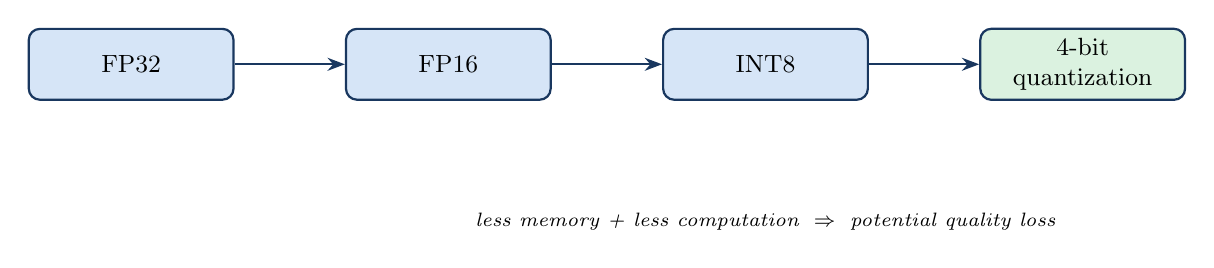
\begin{tikzpicture}[node distance=1.4cm]
\node[block] (fp32) {FP32};
\node[block, right=of fp32] (fp16) {FP16};
\node[block, right=of fp16] (int8) {INT8};
\node[blockgreen, right=of int8] (q4) {4-bit \\ quantization};
\foreach \a/\b in {fp32/fp16, fp16/int8, int8/q4}
  \draw[arrow] (\a) -- (\b);
\node[label, below=1.3cm of int8, align=center] {less memory + less computation $\;\Rightarrow\;$ potential quality loss};
\end{tikzpicture}
\caption{Progressive precision reduction. Q4\_K\_M is not a file-compression trick; it changes how inference is performed.}
\end{figure}

\subsubsection{Warm Context}

\begin{figure}[h]
\centering
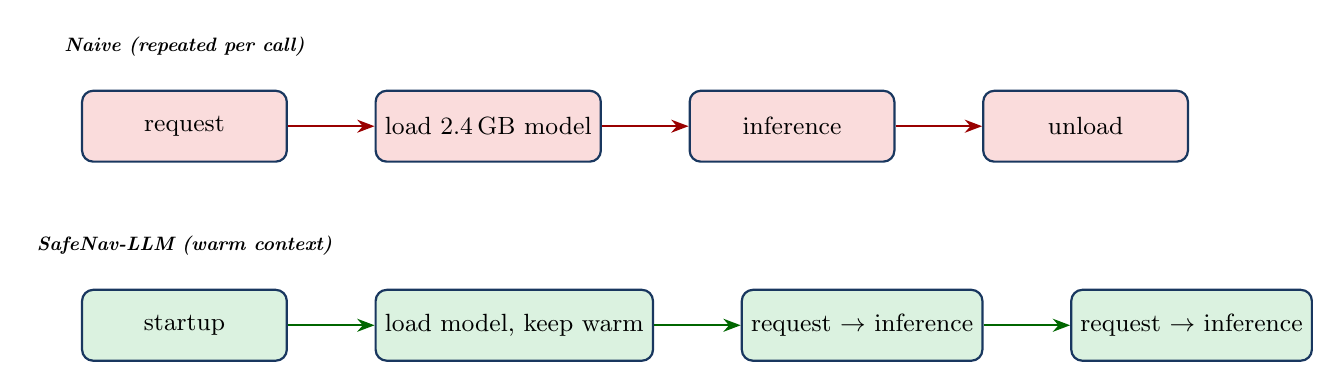
\begin{tikzpicture}[node distance=0.5cm and 1.1cm]
\node[blockred] (b1) {request};
\node[blockred, right=of b1] (b2) {load 2.4\,GB model};
\node[blockred, right=of b2] (b3) {inference};
\node[blockred, right=of b3] (b4) {unload};
\foreach \a/\b in {b1/b2, b2/b3, b3/b4}
  \draw[arrowred] (\a) -- (\b);
\node[label, above=0.3cm of b1] {\textbf{Naive (repeated per call)}};

\node[blockgreen, below=1.6cm of b1] (c1) {startup};
\node[blockgreen, right=of c1] (c2) {load model, keep warm};
\node[blockgreen, right=of c2] (c3) {request $\to$ inference};
\node[blockgreen, right=of c3] (c4) {request $\to$ inference};
\foreach \a/\b in {c1/c2, c2/c3, c3/c4}
  \draw[arrowgreen] (\a) -- (\b);
\node[label, above=0.3cm of c1] {\textbf{SafeNav-LLM (warm context)}};
\end{tikzpicture}
\caption{Loading the model once at startup eliminates per-call loading overhead.}
\end{figure}

\subsubsection{Threading}

Running inference directly on the ROS spin thread risks blocking other
callbacks (localization, costmap updates, control) for hundreds of
milliseconds. SafeNav-LLM instead dispatches inference to a dedicated
\texttt{rclcpp::ThreadPool} with two workers.

\begin{figure}[h]
\centering
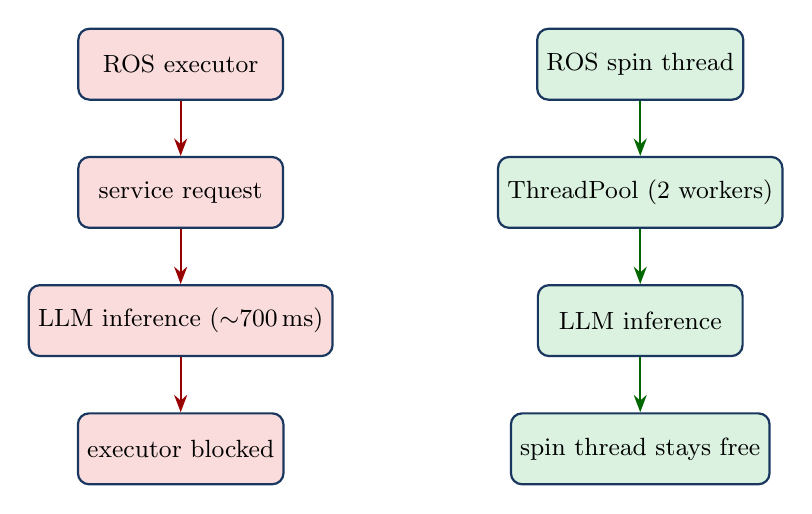
\begin{tikzpicture}[node distance=0.7cm]
\node[blockred] (exec) {ROS executor};
\node[blockred, below=of exec] (req) {service request};
\node[blockred, below=of req] (inf) {LLM inference ($\sim$700\,ms)};
\node[blockred, below=of inf] (blocked) {executor blocked};
\foreach \a/\b in {exec/req, req/inf, inf/blocked}
  \draw[arrowred] (\a) -- (\b);

\node[blockgreen, right=3.2cm of exec] (exec2) {ROS spin thread};
\node[blockgreen, below=of exec2] (pool) {ThreadPool (2 workers)};
\node[blockgreen, below=of pool] (inf2) {LLM inference};
\node[blockgreen, below=of inf2] (free) {spin thread stays free};
\foreach \a/\b in {exec2/pool, pool/inf2, inf2/free}
  \draw[arrowgreen] (\a) -- (\b);
\end{tikzpicture}
\caption{Blocking inference on the executor thread (left) versus offloading to a thread pool (right, as used in SafeNav-LLM).}
\end{figure}

\subsection{Framing of Gap A}
\gapbox{What Gap A actually means}{
The gap is \emph{not} that nobody has run an LLM locally --- prior work such as
LocalNav already demonstrates on-device LLM/VLM inference. Rather:
\emph{existing work demonstrates that on-device inference is feasible, but does
not combine it with the specific semantic waypoint safety boundary, native
Nav2 BT integration, and deployment-specific calibration of SafeNav-LLM.}
}

% ============================================================================
\section{Gap B --- Closed-Set Named-Node Output as a Structural Safety Boundary}
\label{sec:gapb}

\subsection{Open-Vocabulary Risk}

An ordinary LLM has a huge vocabulary and can generate room names that do not
exist in the building, because language models know language --- not the
authoritative world state of a particular building.

\begin{table}[h]
\centering
\begin{tabular}{ll}
\toprule
\textbf{Known rooms (graph)} & \textbf{Possible LLM output} \\
\midrule
Kitchen & Cafeteria \\
Server Room & Laboratory \\
Charging Dock & Warehouse \\
Reception & ICU, Storage Annex \\
\bottomrule
\end{tabular}
\caption{An unconstrained model can generate rooms outside the known set.}
\end{table}

\subsection{Post-Hoc Validation vs.\ Structural Prevention}

\begin{figure}[h]
\centering
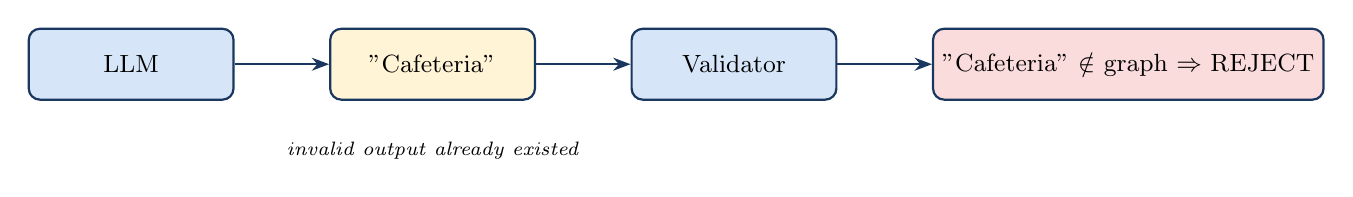
\begin{tikzpicture}[node distance=0.6cm]
\node[block] (llm1) {LLM};
\node[blockyellow, right=1.2cm of llm1] (out1) {"Cafeteria"};
\node[block, right=1.2cm of out1] (val) {Validator};
\node[blockred, right=1.2cm of val] (rej) {"Cafeteria" $\notin$ graph $\Rightarrow$ REJECT};
\foreach \a/\b in {llm1/out1, out1/val, val/rej}
  \draw[arrow] (\a) -- (\b);
\node[label, below=0.4cm of out1] {invalid output already existed};
\end{tikzpicture}
\caption{Post-hoc validation (e.g.\ as used in SPINE) rejects invalid output only \emph{after} it has been generated.}
\end{figure}

SafeNav-LLM instead constrains the \emph{generation grammar itself} so that
invalid names are not merely rejected --- they are not a reachable generation
path:

\begin{lstlisting}[caption={GBNF-style structural constraint on room values}]
Allowed rooms = { kitchen, server_room, charging_dock, reception }

room-value ::=
    "kitchen"
  | "server_room"
  | "charging_dock"
  | "reception"
\end{lstlisting}

\subsection{Token-Level Constraint}

LLMs generate text sequentially, producing a probability distribution
$P(\text{token}\mid\text{previous tokens})$ at each step. A constrained decoder
restricts the \emph{support} of this distribution before sampling:

\begin{figure}[h]
\centering
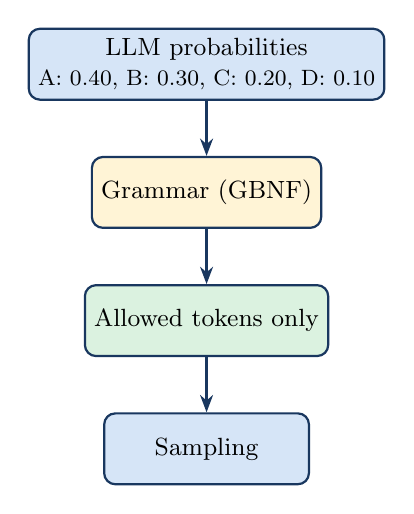
\begin{tikzpicture}[node distance=0.7cm]
\node[block] (probs) {LLM probabilities \\ \footnotesize A: 0.40, B: 0.30, C: 0.20, D: 0.10};
\node[blockyellow, below=of probs] (gram) {Grammar (GBNF)};
\node[blockgreen, below=of gram] (allowed) {Allowed tokens only};
\node[block, below=of allowed] (sample) {Sampling};
\foreach \a/\b in {probs/gram, gram/allowed, allowed/sample}
  \draw[arrow] (\a) -- (\b);
\end{tikzpicture}
\caption{Grammar constraints act \emph{during} generation, at the token-sampler level, rather than after a finished answer is produced.}
\end{figure}

\subsection{Why Names Instead of Coordinates}

Allowing the LLM to emit raw coordinates (\texttt{x}, \texttt{y}, $\theta$)
would make it participate in unconstrained geometry generation. Instead, the
LLM only selects a semantic label; a deterministic lookup resolves the pose.

\begin{figure}[h]
\centering
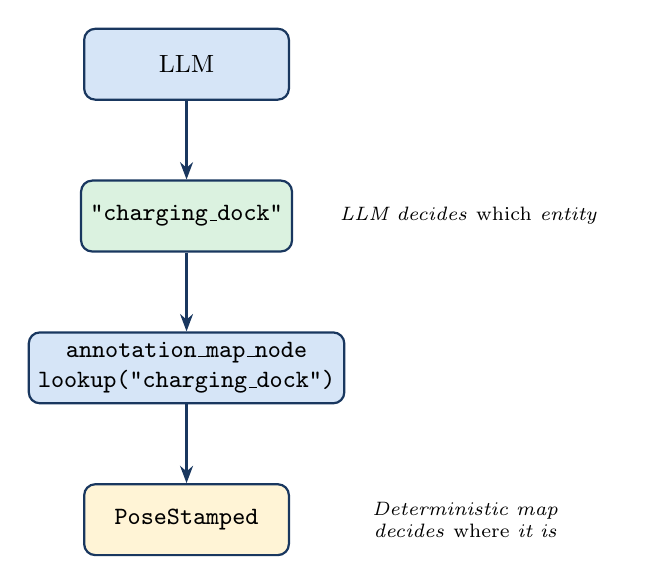
\begin{tikzpicture}[node distance=1.0cm]
\node[block] (llm) {LLM};
\node[blockgreen, below=of llm] (name) {\texttt{"charging\_dock"}};
\node[block, below=of name] (lookup) {\texttt{annotation\_map\_node} \\ \texttt{lookup("charging\_dock")}};
\node[blockyellow, below=of lookup] (pose) {\texttt{PoseStamped}};
\foreach \a/\b in {llm/name, name/lookup, lookup/pose}
  \draw[arrow] (\a) -- (\b);
\node[label, right=0.3cm of name, text width=3.6cm] {LLM decides \emph{which} entity};
\node[label, right=0.3cm of pose, text width=3.6cm] {Deterministic map decides \emph{where} it is};
\end{tikzpicture}
\caption{Separation of responsibilities: semantic selection (LLM) versus deterministic coordinate lookup (annotation graph).}
\end{figure}

\begin{lstlisting}[caption={Annotation graph entry: a deterministic name-to-pose mapping}]
{
  "name": "charging_dock",
  "aliases": ["charging station", "dock", "charger", "power point"],
  "pose": { "x": 3.2, "y": -1.1, "theta": 1.57, "frame": "map" }
}
\end{lstlisting}

\subsection{The Annotation Graph as a Safety Boundary}

\begin{figure}[h]
\centering
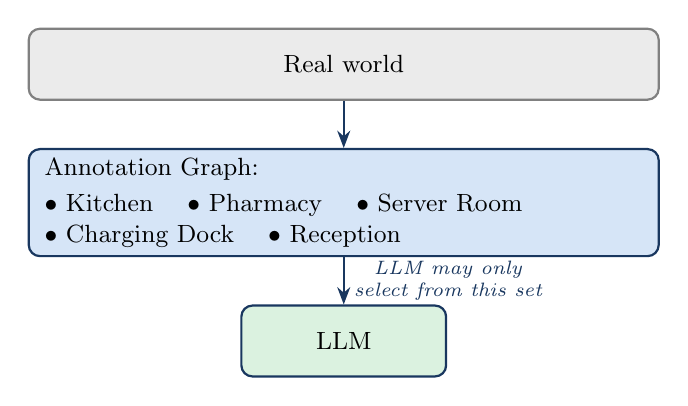
\begin{tikzpicture}[node distance=0.6cm]
\node[blockgray, minimum width=8cm] (world) {Real world};
\node[block, below=of world, minimum width=8cm, align=left,
      text width=7.6cm] (graph) {Annotation Graph:\\[2pt]
      $\bullet$ Kitchen \quad $\bullet$ Pharmacy \quad $\bullet$ Server Room \\
      $\bullet$ Charging Dock \quad $\bullet$ Reception};
\node[blockgreen, below=of graph] (llm) {LLM};
\draw[arrow] (world) -- (graph);
\draw[arrow] (graph) -- (llm) node[midway,right,label]{LLM may only\\select from this set};
\end{tikzpicture}
\caption{The annotation graph forms a bounded semantic universe between unbounded language generation and bounded robot action.}
\end{figure}

\gapbox{Does the closed set guarantee physical safety?}{
\textbf{No.} A closed-set constraint guarantees that the generated semantic
location belongs to the validated set. It does \emph{not} guarantee the robot
cannot collide --- the annotation itself could be stale, an obstacle could have
moved, or the map could be outdated. Nav2's planners, costmaps, and
localization remain responsible for actual motion safety. The correct claim
is narrower: \emph{the closed set structurally prevents out-of-graph
semantic/coordinate hallucination from the LLM} --- one safety layer among
several, not the entire safety system.
}

\subsection{Aliases and Spatial Relationships}

The graph stores linguistic variants that all resolve to one canonical node,
and can encode spatial edges (e.g.\ \emph{adjacent}) enabling relational
commands such as ``the room next to the charging dock.''

\begin{figure}[h]
\centering
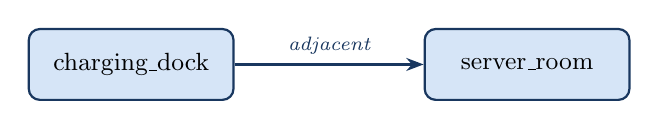
\begin{tikzpicture}[node distance=2.4cm]
\node[block] (dock) {charging\_dock};
\node[block, right=of dock] (server) {server\_room};
\draw[arrow] (dock) -- node[above,label]{adjacent} (server);
\end{tikzpicture}
\caption{Spatial-relationship edges allow relational natural-language commands while keeping physical locations in the graph.}
\end{figure}

% ============================================================================
\section{Gap C --- LLM Inference Inside a Native Nav2 BehaviorTree Node}
\label{sec:gapc}

\subsection{BehaviorTree Basics}

A BehaviorTree is a hierarchical decision/execution structure. Nodes return
one of \texttt{SUCCESS}, \texttt{FAILURE}, or \texttt{RUNNING}.

\begin{figure}[h]
\centering
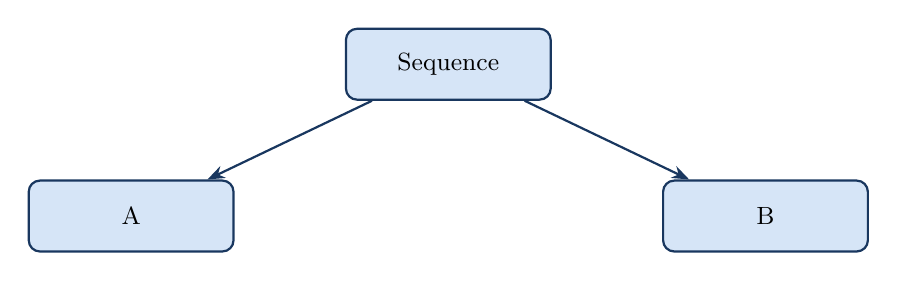
\begin{tikzpicture}[node distance=1.0cm and 1.4cm]
\node[block] (seq) {Sequence};
\node[block, below left=of seq] (a) {A};
\node[block, below right=of seq] (b) {B};
\draw[arrow] (seq) -- (a);
\draw[arrow] (seq) -- (b);
\end{tikzpicture}
\caption{A \texttt{Sequence} executes A, then B only if A succeeds.}
\end{figure}

\begin{figure}[h]
\centering
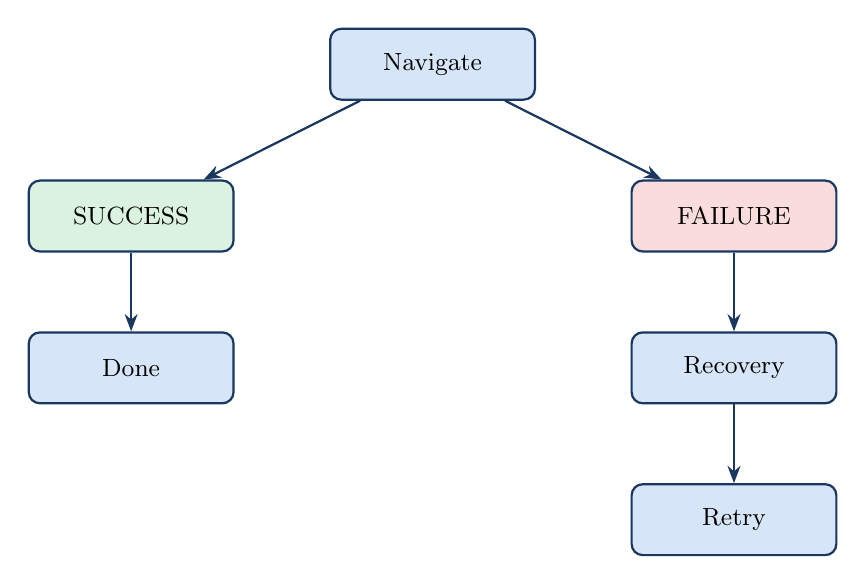
\begin{tikzpicture}[node distance=1.0cm and 1.2cm]
\node[block] (nav) {Navigate};
\node[blockgreen, below left=of nav] (succ) {SUCCESS};
\node[blockred, below right=of nav] (fail) {FAILURE};
\node[block, below=of succ] (done) {Done};
\node[block, below=of fail] (rec) {Recovery};
\node[block, below=of rec] (retry) {Retry};
\draw[arrow] (nav) -- (succ);
\draw[arrow] (nav) -- (fail);
\draw[arrow] (succ) -- (done);
\draw[arrow] (fail) -- (rec);
\draw[arrow] (rec) -- (retry);
\end{tikzpicture}
\caption{BehaviorTrees naturally express navigate--recover--retry mission logic.}
\end{figure}

\subsection{External LLM vs.\ Native Plugin Architecture}

\begin{figure}[h]
\centering
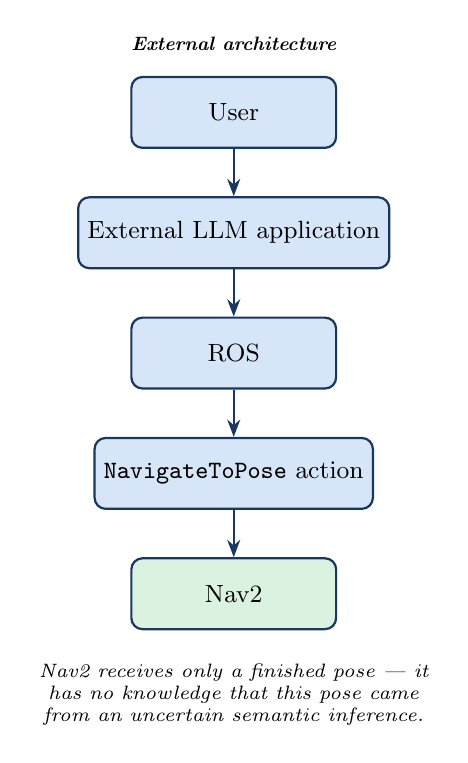
\begin{tikzpicture}[node distance=0.6cm]
\node[block] (u1) {User};
\node[block, below=of u1] (ext) {External LLM application};
\node[block, below=of ext] (ros1) {ROS};
\node[block, below=of ros1] (act) {\texttt{NavigateToPose} action};
\node[blockgreen, below=of act] (nav2a) {Nav2};
\foreach \a/\b in {u1/ext, ext/ros1, ros1/act, act/nav2a}
  \draw[arrow] (\a) -- (\b);
\node[label, above=0.2cm of u1]{\textbf{External architecture}};
\node[label, below=0.3cm of nav2a, text width=5cm]{Nav2 receives only a finished pose --- it has no knowledge that this pose came from an uncertain semantic inference.};
\end{tikzpicture}
\caption{In an external-LLM architecture, semantic resolution happens entirely outside Nav2's execution graph.}
\end{figure}

\begin{figure}[h]
\centering
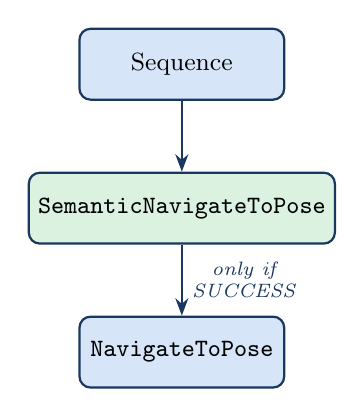
\begin{tikzpicture}[node distance=0.9cm]
\node[block] (seq) {Sequence};
\node[blockgreen, below=of seq] (snp) {\texttt{SemanticNavigateToPose}};
\node[block, below=of snp] (np) {\texttt{NavigateToPose}};
\draw[arrow] (seq) -- (snp);
\draw[arrow] (snp) -- (np) node[midway,right,label]{only if\\SUCCESS};
\end{tikzpicture}
\caption{Native architecture: semantic resolution is itself a BehaviorTree action node, gating the rest of the tree.}
\end{figure}

\subsection{Plugin Integration}

The plugin inherits from \texttt{BT::ActionNodeBase} and is loaded via
\texttt{pluginlib} without modifying Nav2 source:

\begin{figure}[h]
\centering
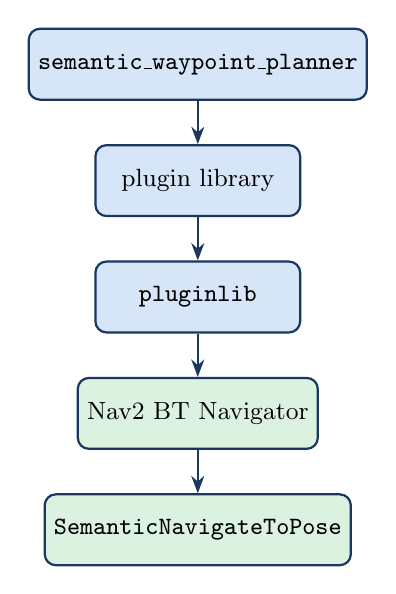
\begin{tikzpicture}[node distance=0.55cm]
\node[block] (pkg) {\texttt{semantic\_waypoint\_planner}};
\node[block, below=of pkg] (lib) {plugin library};
\node[block, below=of lib] (pluginlib) {\texttt{pluginlib}};
\node[blockgreen, below=of pluginlib] (nav2bt) {Nav2 BT Navigator};
\node[blockgreen, below=of nav2bt] (node) {\texttt{SemanticNavigateToPose}};
\foreach \a/\b in {pkg/lib, lib/pluginlib, pluginlib/nav2bt, nav2bt/node}
  \draw[arrow] (\a) -- (\b);
\end{tikzpicture}
\caption{Loading path from the compiled plugin library into the running Nav2 BT Navigator.}
\end{figure}

\begin{lstlisting}[language=, caption={The only Nav2 configuration change required}]
plugin_lib_names:
  - semantic_waypoint_planner
\end{lstlisting}

Because the node participates natively in the tree, it gains: tick timing,
status propagation (\texttt{SUCCESS}/\texttt{FAILURE}), blackboard read/write
access, fallback-branch triggering, configurable timeouts, and direct control
over mission continuation.

\subsection{The Blackboard}

\begin{figure}[h]
\centering
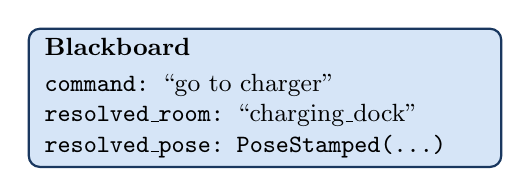
\begin{tikzpicture}
\node[block, minimum width=6cm, align=left, text width=5.6cm] (bb)
 {\textbf{Blackboard}\\[2pt]
  \texttt{command:} ``go to charger''\\
  \texttt{resolved\_room:} ``charging\_dock''\\
  \texttt{resolved\_pose:} \texttt{PoseStamped(...)}};
\end{tikzpicture}
\caption{Shared state written by the semantic node and consumed by downstream BT nodes.}
\end{figure}

\subsection{The Seven-Step Tick Sequence}

\begin{figure}[h]
\centering
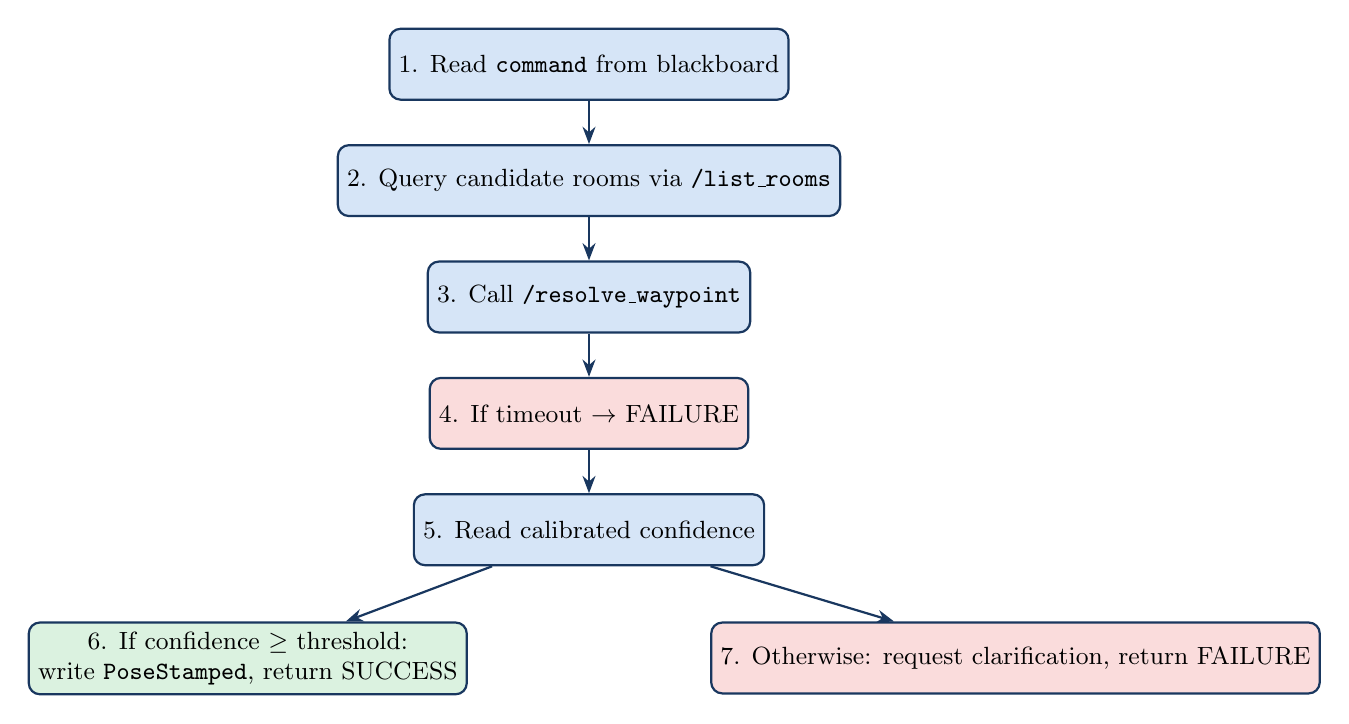
\begin{tikzpicture}[node distance=0.55cm]
\node[block] (s1) {1. Read \texttt{command} from blackboard};
\node[block, below=of s1] (s2) {2. Query candidate rooms via \texttt{/list\_rooms}};
\node[block, below=of s2] (s3) {3. Call \texttt{/resolve\_waypoint}};
\node[blockred, below=of s3] (s4) {4. If timeout $\to$ FAILURE};
\node[block, below=of s4] (s5) {5. Read calibrated confidence};
\node[blockgreen, below left=0.7cm and -0.7cm of s5] (s6) {6. If confidence $\geq$ threshold: \\ write \texttt{PoseStamped}, return SUCCESS};
\node[blockred, below right=0.7cm and -0.7cm of s5] (s7) {7. Otherwise: request clarification, return FAILURE};
\foreach \a/\b in {s1/s2, s2/s3, s3/s4, s4/s5}
  \draw[arrow] (\a) -- (\b);
\draw[arrow] (s5) -- (s6);
\draw[arrow] (s5) -- (s7);
\end{tikzpicture}
\caption{The \texttt{SemanticNavigateToPose} tick logic, as specified in the Phase 2 design.}
\end{figure}

\gapbox{Why FAILURE is useful}{
When resolution confidence is low, the system does not force a guess.
\texttt{SemanticNavigateToPose} returns \texttt{FAILURE}, the BT fallback
subtree runs a \texttt{SpeakText} clarification node, and the tree becomes
part of the \emph{uncertainty-management mechanism} rather than a passive
executor of possibly-wrong poses.
}

\subsection{Comparison with BTGenBot}

\begin{figure}[h]
\centering
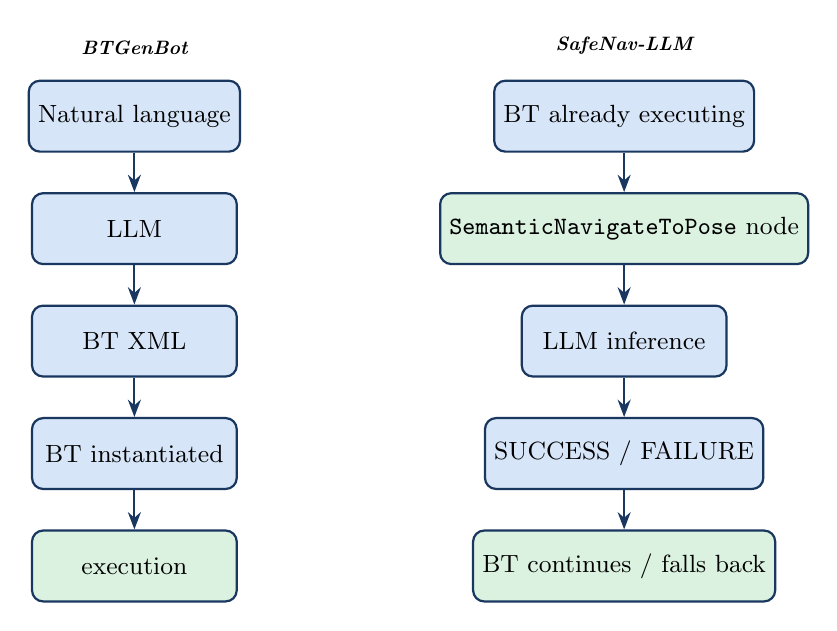
\begin{tikzpicture}[node distance=0.5cm]
\node[block] (nl1) {Natural language};
\node[block, below=of nl1] (llmg) {LLM};
\node[block, below=of llmg] (xml) {BT XML};
\node[block, below=of xml] (inst) {BT instantiated};
\node[blockgreen, below=of inst] (exec1) {execution};
\foreach \a/\b in {nl1/llmg, llmg/xml, xml/inst, inst/exec1}
  \draw[arrow] (\a) -- (\b);
\node[label, above=0.2cm of nl1] {\textbf{BTGenBot}};

\node[block, right=3.2cm of nl1] (bt2) {BT already executing};
\node[blockgreen, below=of bt2] (snode) {\texttt{SemanticNavigateToPose} node};
\node[block, below=of snode] (llm2) {LLM inference};
\node[block, below=of llm2] (res2) {SUCCESS / FAILURE};
\node[blockgreen, below=of res2] (cont) {BT continues / falls back};
\foreach \a/\b in {bt2/snode, snode/llm2, llm2/res2, res2/cont}
  \draw[arrow] (\a) -- (\b);
\node[label, above=0.2cm of bt2] {\textbf{SafeNav-LLM}};
\end{tikzpicture}
\caption{BTGenBot's LLM generates a tree \emph{before} execution; SafeNav-LLM's LLM runs \emph{inside} a live tree action node.}
\end{figure}

% ============================================================================
\section{Gap D --- Deployment-Log-Trained Confidence Calibration}
\label{sec:gapd}

\subsection{Calibration vs.\ Accuracy}

\begin{table}[h]
\centering
\begin{tabular}{lccc}
\toprule
& \textbf{Trials} & \textbf{Correct} & \textbf{Rate} \\
\midrule
Accuracy (raw)          & 100 & 85 & 85\% \\
Confidence $\approx$ 0.9 (subset) & 100 & 70 & 70\% (overconfident) \\
\bottomrule
\end{tabular}
\caption{Accuracy asks how often the model is correct; calibration asks whether confidence values match actual correctness frequency.}
\end{table}

\begin{figure}[h]
\centering
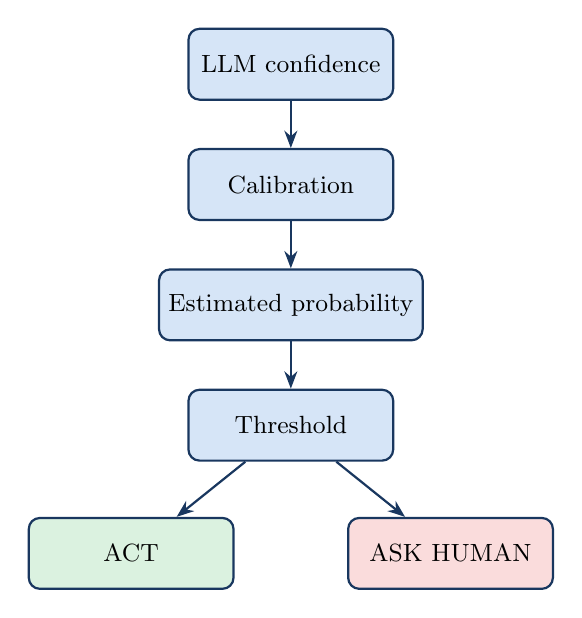
\begin{tikzpicture}[node distance=0.6cm]
\node[block] (conf) {LLM confidence};
\node[block, below=of conf] (cal) {Calibration};
\node[block, below=of cal] (prob) {Estimated probability};
\node[block, below=of prob] (thresh) {Threshold};
\node[blockgreen, below left=0.7cm and -0.6cm of thresh] (act) {ACT};
\node[blockred, below right=0.7cm and -0.6cm of thresh] (ask) {ASK HUMAN};
\foreach \a/\b in {conf/cal, cal/prob, prob/thresh}
  \draw[arrow] (\a) -- (\b);
\draw[arrow] (thresh) -- (act);
\draw[arrow] (thresh) -- (ask);
\end{tikzpicture}
\caption{Calibration converts a vague confidence number into an operational safety decision.}
\end{figure}

\subsection{Deployment-Specific Calibration}

The same LLM, deployed in two different buildings, faces different
uncertainty distributions: exact room names in one building versus vague
relational phrasing (``the lab next to the server area'') in another.
General LLM confidence therefore does not equal deployment-specific
reliability. SafeNav-LLM collects 5 users $\times$ 40 commands = 200 trials
from the actual deployment as its calibration training set.

\subsection{The Five Calibration Features}

\begin{table}[h]
\centering
\begin{tabular}{@{}p{3.2cm}p{9.6cm}@{}}
\toprule
\textbf{Feature} & \textbf{Description} \\
\midrule
Raw LLM confidence & The model's self-reported score, e.g.\ 0.91 --- learned to be predictive or not. \\
Token entropy & Concentration of the output distribution; low entropy (e.g.\ 0.95/0.02/0.02/0.01) signals confident selection, high entropy (e.g.\ 0.35/0.30/0.20/0.15) signals ambiguity. \\
Candidate room count & Size of the semantic search space (e.g.\ 3 rooms vs.\ 30 rooms). \\
Command length & Longer, more structurally complex commands can correlate with resolution difficulty. \\
Levenshtein distance & Minimum edit distance between the resolved room name and a substring of the command --- captures lexical similarity (or its absence). \\
\bottomrule
\end{tabular}
\caption{The five deployment features used by the calibrator.}
\end{table}

\subsection{Platt-Scaled Logistic Regression}

\[
\mathbf{x} = [\,\text{raw\_confidence},\ \text{entropy},\ \text{candidate\_count},\ \text{command\_length},\ \text{edit\_distance}\,]
\]
\[
P(\text{correct}\mid \mathbf{x}) = \sigma\!\left(w^\top \mathbf{x} + b\right), \qquad \sigma(z) = \frac{1}{1+e^{-z}}
\]

\begin{figure}[h]
\centering
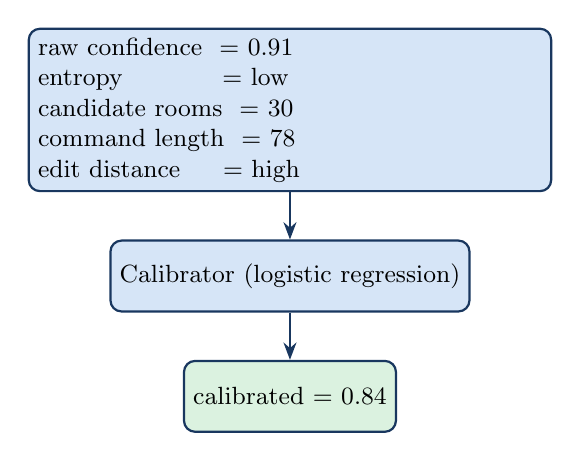
\begin{tikzpicture}[node distance=0.6cm]
\node[block, align=left, text width=6.4cm] (feat)
 {raw confidence \ = 0.91\\
  entropy \hspace{1.05cm} = low\\
  candidate rooms \ = 30\\
  command length \ = 78\\
  edit distance \ \ \ \ = high};
\node[block, below=of feat] (calmodel) {Calibrator (logistic regression)};
\node[blockgreen, below=of calmodel] (out) {calibrated = 0.84};
\draw[arrow] (feat) -- (calmodel);
\draw[arrow] (calmodel) -- (out);
\end{tikzpicture}
\caption{Feature vector combined via Platt-scaled logistic regression into a calibrated probability, which is far more useful as a decision variable than the raw 0.91.}
\end{figure}

\subsection{Expected Calibration Error (ECE)}

\begin{table}[h]
\centering
\begin{tabular}{lc}
\toprule
\textbf{Confidence bin} & \textbf{Actual accuracy} \\
\midrule
0.5--0.6 & 0.54 \\
0.6--0.7 & 0.68 \\
0.7--0.8 & 0.75 \\
0.8--0.9 & 0.84 \\
0.9--1.0 & 0.91 \\
\bottomrule
\end{tabular}
\caption{Well-calibrated confidence bins track actual accuracy closely. Target: ECE $\leq 0.08$.}
\end{table}

\subsection{Safety Thresholds}

\begin{table}[h]
\centering
\begin{tabular}{lcl}
\toprule
\textbf{Error type} & \textbf{Target} & \textbf{Consequence} \\
\midrule
False pass (SAFE but wrong) & $\leq 5\%$ & Dangerous --- robot acts incorrectly \\
False rejection (UNSAFE but correct) & $\leq 15\%$ & Safer, but annoying --- asks human unnecessarily \\
\bottomrule
\end{tabular}
\caption{Deliberate asymmetric safety tradeoff: rejections are tolerated far more than false passes.}
\end{table}

% ============================================================================
\section{Combining the Gaps}
\label{sec:combine}

\subsection{Gap B + Gap D}

The closed set answers \emph{``Is this a legitimate known location?''}; the
calibrator answers \emph{``Do we trust this particular interpretation?''} ---
two entirely different questions.

\subsection{Gap B + Gap C}

\begin{figure}[h]
\centering
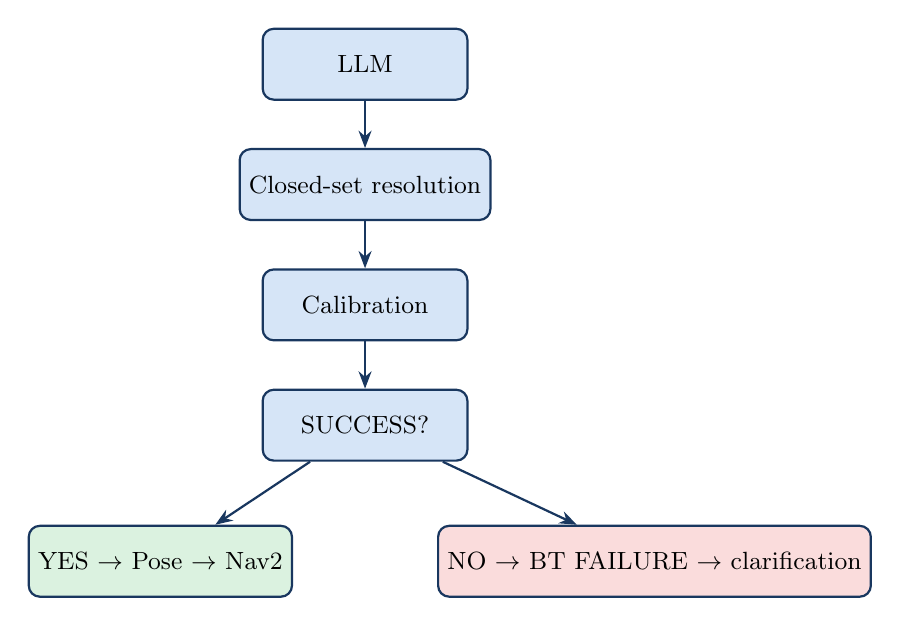
\begin{tikzpicture}[node distance=0.6cm]
\node[block] (llm) {LLM};
\node[block, below=of llm] (cs) {Closed-set resolution};
\node[block, below=of cs] (cal) {Calibration};
\node[block, below=of cal] (dec) {SUCCESS?};
\node[blockgreen, below left=0.8cm and -0.4cm of dec] (yes) {YES $\to$ Pose $\to$ Nav2};
\node[blockred, below right=0.8cm and -0.4cm of dec] (no) {NO $\to$ BT FAILURE $\to$ clarification};
\foreach \a/\b in {llm/cs, cs/cal, cal/dec}
  \draw[arrow] (\a) -- (\b);
\draw[arrow] (dec) -- (yes);
\draw[arrow] (dec) -- (no);
\end{tikzpicture}
\caption{Uncertainty becomes explicit BehaviorTree control flow rather than a silent error.}
\end{figure}

\subsection{Gap A + Gap C}

On-device inference means the BT can operate with a bounded, local timeout
(3000\,ms for the resolver; 5000\,ms default for the broader BT timing
constraint) without depending on an external service.

% ============================================================================
\section{The Complete Architecture}
\label{sec:complete}

\begin{figure}[h!]
\centering
\resizebox{\textwidth}{!}{%
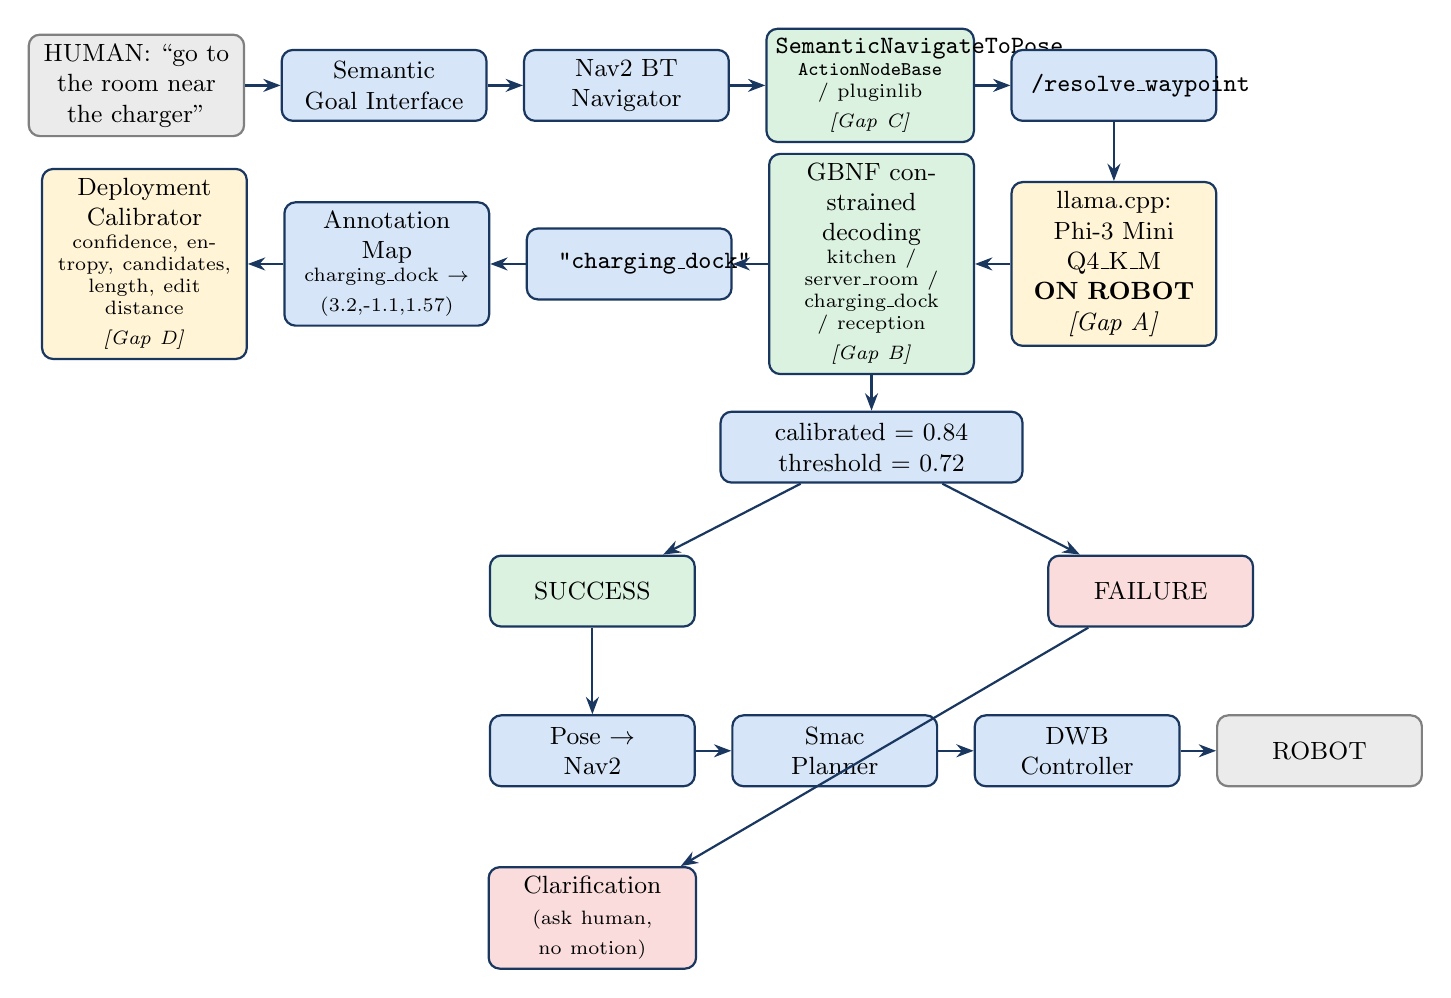
\begin{tikzpicture}[node distance=0.45cm, every node/.style={font=\scriptsize}]

% ---- Row 1: left to right ----
\node[blockgray, text width=2.5cm] (human) {HUMAN: ``go to the room near the charger''};
\node[block, right=of human, text width=2.1cm] (iface) {Semantic Goal Interface};
\node[block, right=of iface, text width=2.0cm] (nav2bt) {Nav2 BT Navigator};
\node[blockgreen, right=of nav2bt, text width=2.4cm] (snp) {\texttt{SemanticNavigateToPose} \\ \scriptsize \texttt{ActionNodeBase} / pluginlib \\ \textit{[Gap C]}};
\node[block, right=of snp, text width=2.1cm] (svc) {\texttt{/resolve\_waypoint}};

% ---- Row 2: right to left (directly below row 1, flowing back) ----
\node[blockyellow, below=0.75cm of svc, text width=2.3cm] (llama) {llama.cpp: Phi-3 Mini Q4\_K\_M \\ \textbf{ON ROBOT} \\ \textit{[Gap A]}};
\node[blockgreen, left=of llama, text width=2.3cm] (grammar) {GBNF constrained decoding \\ \scriptsize kitchen / server\_room / \\ charging\_dock / reception \\ \textit{[Gap B]}};
\node[block, left=of grammar, text width=1.8cm] (name) {\texttt{"charging\_dock"}};
\node[block, left=of name, text width=2.1cm] (amap) {Annotation Map \\ \scriptsize charging\_dock $\to$ \\ (3.2,-1.1,1.57)};
\node[blockyellow, left=of amap, text width=2.3cm] (calib) {Deployment Calibrator \\ \scriptsize confidence, entropy, candidates, \\ length, edit distance \\ \textit{[Gap D]}};

% ---- Row 3: decision, centered under row 2 ----
\node[block, below=of grammar, text width=3.6cm] (calval) {calibrated = 0.84 \quad threshold = 0.72};
\node[blockgreen, below left=0.9cm and 0.3cm of calval] (succ) {SUCCESS};
\node[blockred, below right=0.9cm and 0.3cm of calval] (failn) {FAILURE};
% ---- Row 4: execution chain, left to right ----
\node[block, below=1.1cm of succ, text width=1.9cm] (pose2nav) {Pose $\to$ Nav2};
\node[block, right=of pose2nav, text width=1.9cm] (smac) {Smac Planner};
\node[block, right=of smac, text width=1.9cm] (dwb) {DWB Controller};
\node[blockgray, right=of dwb, text width=1.7cm] (robot) {ROBOT};

% ---- Clarification: placed below the execution row, clear of any overlap ----
\node[blockred, below=1.0cm of pose2nav, text width=2.4cm] (clar) {Clarification \\ \scriptsize (ask human, no motion)};

% ---- Arrows ----
\foreach \a/\b in {human/iface, iface/nav2bt, nav2bt/snp, snp/svc}
  \draw[arrow] (\a) -- (\b);
\draw[arrow] (svc) -- (llama);
\foreach \a/\b in {llama/grammar, grammar/name, name/amap, amap/calib}
  \draw[arrow] (\a) -- (\b);
\draw[arrow] (grammar) -- (calval);
\draw[arrow] (calval) -- (succ);
\draw[arrow] (calval) -- (failn);
\draw[arrow] (failn) -- (clar);
\draw[arrow] (succ) -- (pose2nav);
\draw[arrow] (pose2nav) -- (smac);
\draw[arrow] (smac) -- (dwb);
\draw[arrow] (dwb) -- (robot);
\end{tikzpicture}}
\caption{The complete SafeNav-LLM pipeline, integrating all four architectural gaps. Flow runs left-to-right along the top row, reverses right-to-left through local inference and constrained decoding, then resolves through calibration into either navigation execution or a clarification request.}
\end{figure}

\subsection{What Each Layer Protects Against}

\begin{table}[h]
\centering
\begin{tabular}{@{}p{3.4cm}p{9.4cm}@{}}
\toprule
\textbf{Layer} & \textbf{Main problem it prevents} \\
\midrule
On-device inference (Gap A) & Cloud/network dependency \\
Closed-set decoding (Gap B) & Invented / nonexistent locations \\
Native BT plugin (Gap C) & AI logic disconnected from Nav2's execution semantics \\
Calibration model (Gap D) & Overconfident but incorrect semantic resolutions \\
\bottomrule
\end{tabular}
\caption{Summary role of each architectural gap.}
\end{table}

\gapbox{The four questions}{
\textbf{Gap A:} Can the robot think locally?\\
\textbf{Gap B:} Can it be prevented from inventing places?\\
\textbf{Gap C:} Can that reasoning become a native part of robot execution?\\
\textbf{Gap D:} Can the robot know when it should \emph{not} trust its interpretation?
}

\subsection{Why All Four Are Needed}

\begin{table}[h]
\centering
\begin{tabular}{@{}p{2.1cm}p{10.6cm}@{}}
\toprule
\textbf{Removed} & \textbf{Consequence} \\
\midrule
Gap A & Safe semantic resolver, but the robot cannot function offline. \\
Gap B & LLM may still generate an invalid entity (e.g.\ ``cafeteria''); calibration alone cannot prevent an invalid entity from being generated. \\
Gap C & Semantic system lives outside Nav2; native BT status propagation, blackboard integration, and fallback trees are lost. \\
Gap D & A wrong \emph{but valid} room can still be executed --- the closed-set constraint cannot catch semantically valid misinterpretation. \\
\bottomrule
\end{tabular}
\caption{Removing any single gap reintroduces a distinct failure mode.}
\end{table}

% ============================================================================
\section{Two Failure Types}
\label{sec:failures}

\begin{figure}[h]
\centering
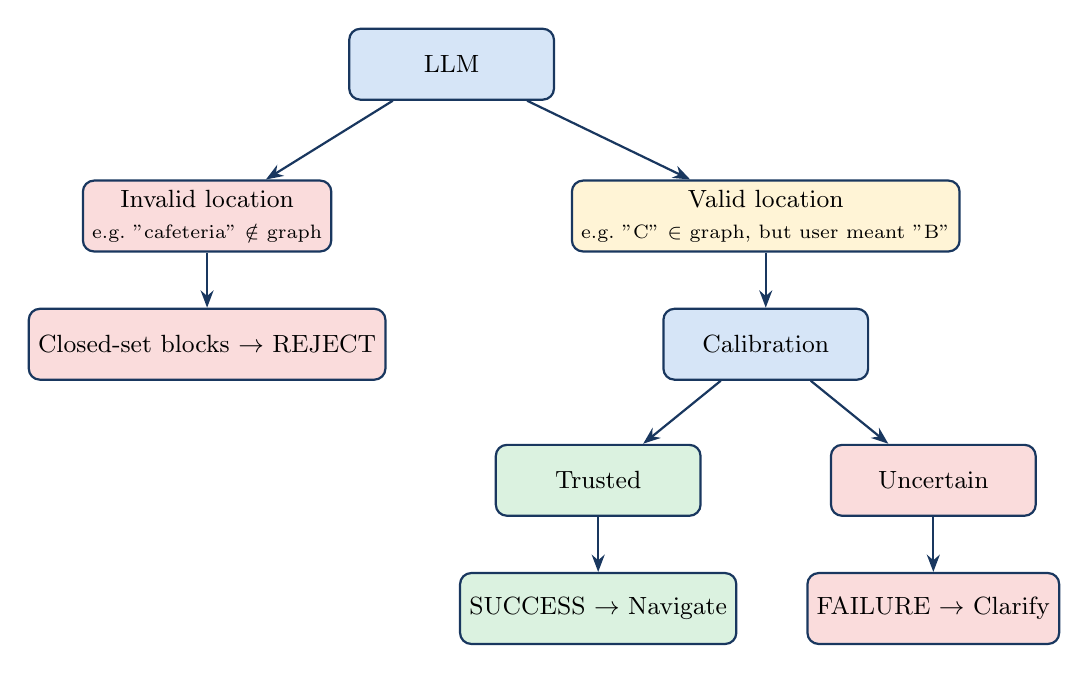
\begin{tikzpicture}[node distance=0.7cm]
\node[block] (llm) {LLM};
\node[blockred, below left=1.0cm and 0.2cm of llm] (inv) {Invalid location \\ \scriptsize e.g.\ "cafeteria" $\notin$ graph};
\node[blockyellow, below right=1.0cm and 0.2cm of llm] (val) {Valid location \\ \scriptsize e.g.\ "C" $\in$ graph, but user meant "B"};
\node[blockred, below=of inv] (block) {Closed-set blocks $\to$ REJECT};
\node[block, below=of val] (calpath) {Calibration};
\node[blockgreen, below left=0.8cm and -0.5cm of calpath] (trust) {Trusted};
\node[blockred, below right=0.8cm and -0.5cm of calpath] (unc) {Uncertain};
\node[blockgreen, below=of trust] (succ2) {SUCCESS $\to$ Navigate};
\node[blockred, below=of unc] (fail2) {FAILURE $\to$ Clarify};

\draw[arrow] (llm) -- (inv);
\draw[arrow] (llm) -- (val);
\draw[arrow] (inv) -- (block);
\draw[arrow] (val) -- (calpath);
\draw[arrow] (calpath) -- (trust);
\draw[arrow] (calpath) -- (unc);
\draw[arrow] (trust) -- (succ2);
\draw[arrow] (unc) -- (fail2);
\end{tikzpicture}
\caption{Two distinct failure types require two distinct solutions: closed-set constraint prevents \emph{invalid-world hallucination}; calibration handles \emph{valid-world misinterpretation}.}
\end{figure}

\begin{table}[h]
\centering
\begin{tabular}{@{}p{3.6cm}p{4.5cm}p{4.5cm}@{}}
\toprule
& \textbf{Failure Type 1} & \textbf{Failure Type 2} \\
\midrule
Name & Invalid-world hallucination & Valid-world misinterpretation \\
Example & User says ``cafeteria''; LLM outputs ``cafeteria'' $\notin$ graph & User means room B; LLM confidently outputs room C, which exists \\
Caught by closed set? & Yes & No --- C is a legitimate node \\
Solution & Closed-set constrained decoding (Gap B) & Confidence calibration + thresholding (Gap D) \\
\bottomrule
\end{tabular}
\caption{Why both Gap B and Gap D are independently necessary.}
\end{table}

% ============================================================================
\section{Defense in Depth}
\label{sec:defense}

\begin{figure}[h]
\centering
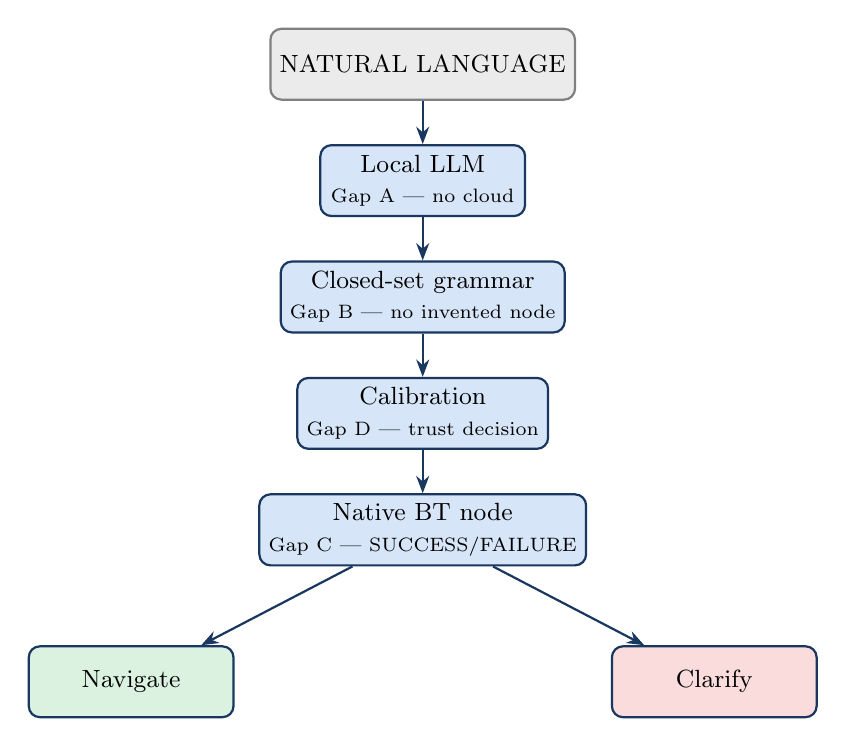
\begin{tikzpicture}[node distance=0.55cm]
\node[blockgray] (nl) {NATURAL LANGUAGE};
\node[block, below=of nl] (a) {Local LLM \\ \scriptsize Gap A --- no cloud};
\node[block, below=of a] (b) {Closed-set grammar \\ \scriptsize Gap B --- no invented node};
\node[block, below=of b] (d) {Calibration \\ \scriptsize Gap D --- trust decision};
\node[block, below=of d] (c) {Native BT node \\ \scriptsize Gap C --- SUCCESS/FAILURE};
\node[blockgreen, below left=1.0cm and 0.3cm of c] (nvg) {Navigate};
\node[blockred, below right=1.0cm and 0.3cm of c] (clr) {Clarify};

\foreach \a/\b in {nl/a, a/b, b/d, d/c}
  \draw[arrow] (\a) -- (\b);
\draw[arrow] (c) -- (nvg);
\draw[arrow] (c) -- (clr);
\end{tikzpicture}
\caption{The four gaps as sequential layers of defense, each with a distinct responsibility.}
\end{figure}

\begin{center}
\begin{tabular}{ll}
\textbf{Gap A} & controls \emph{where} computation happens. \\
\textbf{Gap B} & controls \emph{what} the model is allowed to output. \\
\textbf{Gap D} & controls \emph{whether} the output is trusted. \\
\textbf{Gap C} & controls \emph{how} the robot acts on that decision. \\
\end{tabular}
\end{center}

% ============================================================================
\section{Positioning Against the Literature}
\label{sec:lit}

\begin{table}[h!]
\centering
\small
\begin{tabular}{@{}p{2.3cm}p{5.3cm}p{5.5cm}@{}}
\toprule
\textbf{System} & \textbf{Contribution} & \textbf{Gap relative to SafeNav-LLM} \\
\midrule
LM-Nav & LLM + navigation + graph-based restriction & Cloud GPT-3; no deployment calibration; not Nav2-native; outdoor focus \\
SayCan & LLM + closed skill set + physical feasibility & Cloud PaLM; skill repertoire rather than annotation graph; manipulation focus \\
NLMap & Open-vocabulary semantic navigation & Argues \emph{against} a closed set --- opposite safety philosophy \\
Das et al. & LLM + ROS2 + Nav2 navigation & Cloud models; free-form intent; no calibration; external Nav2 wrapper \\
BTGenBot & LLM + BehaviorTree + Jetson + Nav2 & LLM generates BT XML \emph{before} execution, not embedded in a running plugin node \\
KnowNo & Uncertainty + human clarification & Conformal prediction, not deployment-log-trained supervised calibration \\
SPINE & LLM navigation + safety validation & Safety mechanism is post-hoc, not generation-time constrained \\
LocalNav & On-device model on Jetson + navigation & No closed-set/Nav2-BT/calibration combination \\
osmAG-LLM & Named semantic nodes, no coordinates, constrained output & Most structurally similar prior system --- missing BT/pluginlib integration and deployment calibration \\
\bottomrule
\end{tabular}
\caption{Positioning of SafeNav-LLM relative to closely related prior systems.}
\end{table}

\gapbox{The precise novelty claim}{
osmAG-LLM already restricts an LLM to named semantic nodes, so SafeNav-LLM
cannot claim that restriction as novel in isolation. The stronger claim is the
\emph{combination}:
\begin{center}
osmAG-like semantic restriction $+$ token-level grammar enforcement $+$
explicit safety-boundary framing $+$ on-device inference $+$ native Nav2 BT
pluginlib node $+$ deployment-log calibration.
\end{center}
The contribution is not that any individual component --- local LLMs,
closed-set semantic navigation, BehaviorTrees, or calibration --- is
unprecedented. The research gap is the absence, in the reviewed literature,
of a system that combines all four in a single native Nav2 architecture.
}

% ============================================================================
\section{Precise Claims for Written and Oral Defense}
\label{sec:viva}

\begin{tcolorbox}[colback=softyellow,colframe=navyblue,title={Recommended phrasing},fonttitle=\bfseries,breakable]
\textbf{Avoid:} ``Our system prevents the robot from going to an unsafe
location.'' \emph{(too broad)}

\textbf{Prefer:}
\begin{quote}
\itshape ``Our closed-set constraint prevents the language model from
generating a semantic waypoint outside the pre-validated annotation graph,
while the calibrated confidence gate prevents sufficiently uncertain in-graph
resolutions from being passed to Nav2.''
\end{quote}
\begin{quote}
\itshape ``The Nav2 BehaviorTree plugin provides the execution-level
mechanism that converts acceptance into navigation and rejection into
clarification.''
\end{quote}
\begin{quote}
\itshape ``The contribution is not that any individual component --- local
LLMs, closed-set semantic navigation, BehaviorTrees, or calibration --- is
unprecedented. The research gap is the absence, according to the reviewed
literature, of a system that combines all four in a single native Nav2
architecture.''
\end{quote}
\end{tcolorbox}

\end{document}
